% =====================================================================
%  ch02a.tex —— 第 2 章 分析力学（前半；原书 p.6–21，PDF 15–30）
%  覆盖：章首、2.1 Newton 运动定律、2.2 Lagrange 形式、
%        2.3 Legendre 变换、2.4 Legendre–Fenchel 变换（末尾入 2.5）
% =====================================================================
\chapter{分析力学}
% [原文 p.6]
分析力学已有 200 年以上的历史，是辛几何的故乡。这里不打算沿着真实的历史，
概述从分析力学到辛几何的发展脉络。另一方面，也可以把辛流形定义为具有非退化
闭 2 次微分形式的流形，并从那里开始讨论。这在数学上是标准的做法，但本书也不
取这条路径。本章从分析力学讲起，先把（作者认为）其必然性比辛流形更易理解的
泊松流形（Poisson manifold）公理化，然后作为其特殊情形引入辛流形。

\section{Newton 运动定律}

关于质点系的古典力学，Newton 运动定律（Newton's laws of motion）由以下三条
组成：

\begin{description}[leftmargin=7em, labelwidth=6.3em, labelsep=0.7em, itemsep=2pt]
\item[\textbf{第一定律}] 不受力作用的质点作匀速直线运动。
\item[\textbf{第二定律}] 质点受力的作用时，其加速度与该质点所受诸力之和成正比，
  与该质点的质量成反比。
\item[\textbf{第三定律}] 质点 A 对质点 B 施力时，质点 B 也对质点 A 施加大小相同、
  方向相反的力。
\end{description}

第一定律中虽已陈述「匀速直线运动」，但要确定其含义，必须先选取坐标系。在
Newton 力学中，使不受力作用的质点作匀速直线运动的坐标系，称为 \textbf{Galilei
坐标系}（Galilean reference frame）。第一定律所主张的正是 Galilei 坐标系的存在。

% [Tutor Note: 背景：Newton 三定律见于《自然哲学的数学原理》(1687)；第一定律的
% 实质是断言惯性系的存在，而非仅描述一种运动状态。]
\takeaway{Newton 三定律以 Galilei 坐标系为前提；其「力」概念不明、坐标系受限，
正是转向分析力学的动因。}

第二定律是三条运动定律中最重要的，常常把 Newton 运动方程（Newton's equation
of motion）
% [原文 p.7]
\begin{equation}
  \bm{F} = m\frac{\rd^2\bm{x}}{\rd t^2}
  \tag{2.1.1}
\end{equation}
的形式给出。这里 $m$ 是质点的质量（mass），$\bm{F}$ 是作用在质点上的力
（force），而 $\bm{x}$ 是质点在 Galilei 坐标系中的位置（position）。要陈述
第二定律，其前提是第一定律保证 Galilei 坐标系的存在，这自不待言。

第三定律陈述的是作用与反作用定律，它与动量守恒定律等价。据后文将叙述的
Noether 定理，这等价于系统的平移不变性（或者说空间的均匀性）。

这样表述运动定律，无论从哲学上还是实用上都极不令人满意。哲学上不满的最大
理由在于：按这种表述，「力」究竟是什么并不明确。在 Galilei 坐标系中看到质点
并未作匀速直线运动时，也可以把其质量与加速度的乘积定义为「力」，但那样一来
第二定律就等于什么也没说。因此，除 Newton 运动定律之外还需要关于力的定律，
例如关于弹簧的 Hooke 定律、Newton 万有引力定律，或关于点电荷相互作用的
Coulomb 定律。

另一方面，实用上最大的不满在于：可用的坐标系被固定在 Galilei 坐标系。许多
系统具有对称性，取与该系统对称性相符的坐标，理论上更有通盘之见，计算也更简单。
在 Newton 形式的古典力学中，必须先使用 Galilei 坐标写出运动方程，然后再把它
变换到所偏好的坐标。

此外，关于对称性与守恒定律的 Noether 定理，只有借助分析力学才能自然地陈述。
第三定律与动量守恒定律等价，而按 Noether 定理，动量守恒定律等价于系统具有关于
空间平移的对称性（即「物理在平行移动下不变」）。要从 Newton 运动定律中看出这
一事实，几乎是不可能的。

无论如何，先就几个简单的例子写出 Newton 运动方程看看。

\subsection{简谐振动}

% [Tutor Note: 背景：Noether 定理（1918）把连续对称性与守恒量对应起来：时间
% 平移对应能量、空间平移对应动量、旋转对应角动量。]
% [原文 p.8]
图 2.1 所示的，是用弹簧悬挂在空中的重物的上下运动。设时刻 $t$ 时重物的位置
为 $x = x(t)$，则此时的运动方程为

\begin{figure}[htbp]
  \centering
  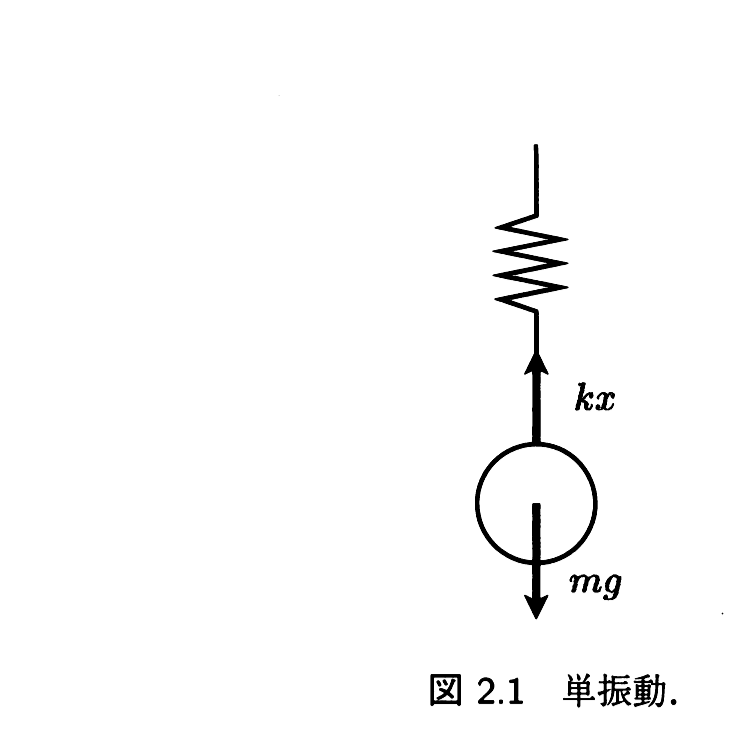
\includegraphics[width=0.40\textwidth,trim=0 19.2bp 0 0,clip]{figures/fig2.1.png}
  \figtitle{2.1}{简谐振动（原书 p.8）}
\end{figure}

\begin{equation}
  m\frac{\rd^2x}{\rd t^2} = -kx - mg
  \tag{2.1.2}
\end{equation}

其中 $m$ 是重物的质量（mass），$k$ 是弹簧常数（stiffness），$g$ 是重力加速度
（gravitational acceleration）。若适当选取时刻 $t$ 与位置 $x$ 的单位，则该方程成为

\begin{equation}
  \frac{\rd^2x}{\rd t^2} = -x - 1
  \tag{2.1.3}
\end{equation}

但这里再令 $y = x + 1$，运动方程便可写成

\begin{equation}
  \frac{\rd^2y}{\rd t^2} = -y
  \tag{2.1.4}
\end{equation}

这是 2 阶线性微分方程，其解空间是由 $\sin t$ 与 $\cos t$ 张成的 2 维线性空间。
这样的运动称为简谐振动（simple harmonic motion）。

\subsection{单摆}

如图 2.2 所示，在半径为 $R$ 的圆周上运动的重物称为单摆（simple gravity
pendulum）。与铅直方向偏离 $\theta$ 的重物所受的力，在 $\theta$ 方向上为
$mg\sin\theta$，运动方程为

\begin{figure}[htbp]
  \centering
  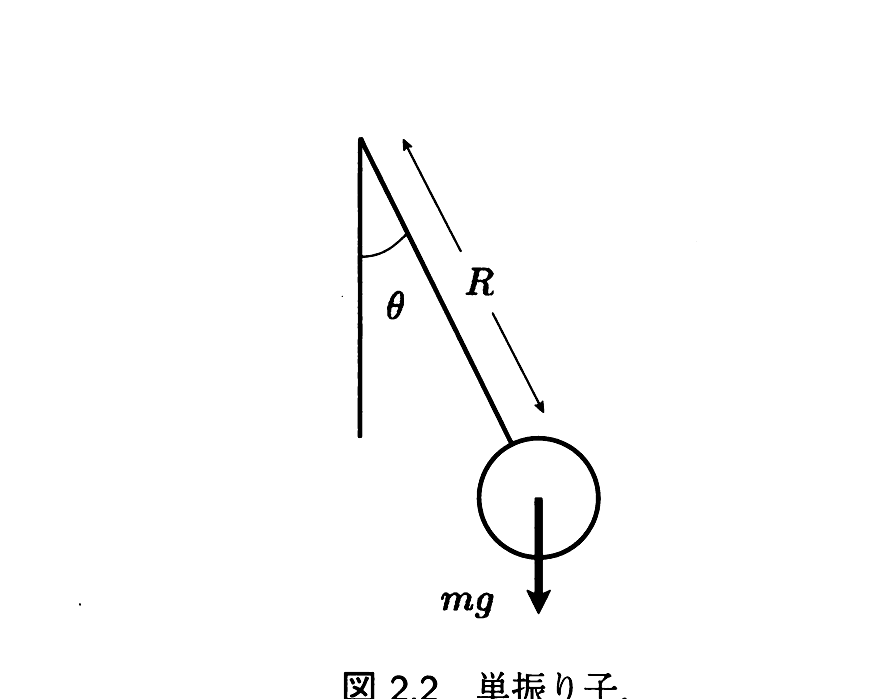
\includegraphics[width=0.42\textwidth,trim=0 6.48bp 0 0,clip]{figures/fig2.2.png}
  \figtitle{2.2}{单摆（原书 p.8）}
\end{figure}

\begin{equation}
  mR\frac{\rd^2\theta}{\rd t^2} = -mg\sin\theta
  \tag{2.1.5}
\end{equation}

适当选取单位制，令 $m = R = g = 1$，并在两边乘以 $\dot\theta$，则

\begin{equation}
  \dot\theta\ddot\theta = -\sin\theta\,\dot\theta
  \tag{2.1.6}
\end{equation}

将上式两边对 $t$ 积分，得

\begin{equation}
  \frac{1}{2}\dot\theta^2 = \cos\theta + E
  \tag{2.1.7}
\end{equation}

这里 $E$ 是积分常数。

\begin{equation}
  E = \frac{1}{2}\dot\theta^2 - \cos\theta
  \tag{2.1.8}
\end{equation}

改写上式，这正是能量守恒定律。把它写成

\begin{equation}
  \frac{\rd\theta}{\rd t} = \sqrt{2(\cos\theta + E)}
  \tag{2.1.9}
\end{equation}

则已成为分离变量形，因此

% [原文 p.9]
\begin{equation}
  \frac{\rd\theta}{\sqrt{2(\cos\theta + E)}} = \rd t
  \tag{2.1.10}
\end{equation}

于是

\begin{equation}
  \int \frac{\rd\theta}{\sqrt{2(\cos\theta + E)}} = t
  \tag{2.1.11}
\end{equation}

由此，$t$ 作为 $\theta$ 的函数被求出，而作为 $t$ 的函数的 $\theta$ 则由其反函数
给出。积分 (2.1.11) 是椭圆积分，其反函数成为椭圆函数。由于方程是非线性的，
解空间不是线性空间；但按常微分方程初值问题解的存在性与唯一性，可由初值（时刻
$t = 0$ 时 $\theta$ 与 $\dot\theta$ 的值）加以参数化。也就是说，解空间是
$S^1 \times \R$。

\subsection{Kepler 问题}

上面两个问题，都是 1 个质点在 1 维空间中运动的问题。由于运动方程是 2 阶常
微分方程，解空间的维数为 2。这里考虑在重力相互作用下于 3 维空间中运动的 2 个
质点。此时解空间的维数为 12，远比前面的例子大得多。然而，这个系统具有很大的
对称性（按 Noether 定理，这等价于守恒定律），所以最终归结为 2 维问题。

% [Tutor Note: 背景：Kepler 问题是二体问题；解空间维数 12，对称性使其约化到
% 质心匀速直线运动（3 维）+ 相对运动的平面轨道（2 维）。]
% [Tutor Note: 难点：(2.1.12) 与 (2.1.13) 中的力大小相同、方向相反，正是第三定律。]
运动方程为

\begin{align}
  m_1\frac{\rd^2\bm{x}_1}{\rd t^2} &= -m_1m_2
    \frac{\bm{x}_1 - \bm{x}_2}{|\bm{x}_1 - \bm{x}_2|^3}, \tag{2.1.12}\\
  m_2\frac{\rd^2\bm{x}_2}{\rd t^2} &= -m_1m_2
    \frac{\bm{x}_2 - \bm{x}_1}{|\bm{x}_2 - \bm{x}_1|^3} \tag{2.1.13}
\end{align}

这里，引入重心的坐标 $\bm{x}'$ 与相对位置 $\bm{x}$：

\begin{align}
  \bm{x}' &= \frac{m_1\bm{x}_1 + m_2\bm{x}_2}{m_1 + m_2}, \tag{2.1.14}\\
  \bm{x} &= \bm{x}_1 - \bm{x}_2 \tag{2.1.15}
\end{align}

则运动方程改写为

\begin{align}
  \ddot{\bm{x}}' &= 0, \tag{2.1.16}\\
  m\ddot{\bm{x}} &= -m_1m_2\frac{\bm{x}}{|\bm{x}|^3} \tag{2.1.17}
\end{align}

这里

\begin{equation}
  m = \frac{m_1m_2}{m_1 + m_2}
  \tag{2.1.18}
\end{equation}

是调和平均的一半，称为约化质量（reduced mass）。(2.1.16) 表明重心作匀速直线
运动。另一方面，(2.1.17) 表明固定质点
% [原文 p.10]
所产生的重力场中运动的 1 个质点的运动方程。适当选取单位制，把它写成

\begin{equation}
  \ddot{\bm{x}} = -\frac{\bm{x}}{|\bm{x}|^3}
  \tag{2.1.19}
\end{equation}

的形式。

3 维向量的外积（cross product）是，对

\begin{align}
  \bm{a} &= (a_1, a_2, a_3), \tag{2.1.20}\\
  \bm{b} &= (b_1, b_2, b_3) \tag{2.1.21}
\end{align}

由

\begin{equation}
  \bm{a}\times\bm{b}
    = (a_2b_3 - a_3b_2,\; a_3b_1 - a_1b_3,\; a_1b_2 - a_2b_1)
  \tag{2.1.22}
\end{equation}

给出。用它定义角动量（angular momentum）

\begin{equation}
  \bm{M} = \bm{x}\times\dot{\bm{x}}
  \tag{2.1.23}
\end{equation}

则

\begin{align}
  \dot{\bm{M}} &= \dot{\bm{x}}\times\dot{\bm{x}}
    + \bm{x}\times\ddot{\bm{x}} \tag{2.1.24}\\
  &= 0 + \bm{x}\times\left(-\frac{\bm{x}}{|\bm{x}|^3}\right) \tag{2.1.25}\\
  &= 0 \tag{2.1.26}
\end{align}

故可知角动量守恒。这里使用了 Leibniz 法则

\begin{equation}
  \frac{\rd}{\rd t}(\bm{a}\times\bm{b})
    = \dot{\bm{a}}\times\bm{b} + \bm{a}\times\dot{\bm{b}}
  \tag{2.1.27}
\end{equation}

与外积的性质

\begin{equation}
  \bm{a}\times\bm{a} = 0
  \tag{2.1.28}
\end{equation}

关于对称性与守恒定律之关系的 Noether 定理主张：角动量守恒定律 $\dot{\bm{M}}=0$
等价于系统的旋转对称性。

% [Tutor Note: 背景：角动量守恒对应旋转对称性，这是 Kepler 第二定律（面积速度
% 一定）的内蕴原因。]
% [Tutor Note: 难点：(2.1.25) 用了 $\dot{\bm{x}}\times\dot{\bm{x}}=0$ 与 (2.1.19)；
% $\bm{x}\times(-\bm{x}/|\bm{x}|^3)=0$ 因两向量共线。]
由外积的定义 (2.1.22) 直接可得

\begin{equation}
  \bm{a}\cdot(\bm{a}\times\bm{b}) = 0
  \tag{2.1.29}
\end{equation}

由此可知，角动量 $\bm{M} := \bm{x}\times\dot{\bm{x}}$ 与 $\bm{x}$ 及
$\dot{\bm{x}}$ 都正交。又因角动量守恒，可知 $\bm{x}$ 始终停留在与 $\bm{M}$
正交的平面内。在这一平面上引入极坐标，写成

\begin{equation}
  \bm{x} = (r\cos\theta, r\sin\theta, 0)
  \tag{2.1.30}
\end{equation}

则角动量为

% [原文 p.11]
\begin{equation}
\begin{aligned}
  \bm{M} &:= \bm{x}\times\dot{\bm{x}}\\
  &= (r\cos\theta,\, r\sin\theta,\, 0)\times
     (\dot r\cos\theta - r\sin\theta\,\dot\theta,\;
      \dot r\sin\theta + r\cos\theta\,\dot\theta,\; 0)\\
  &= (0,\, 0,\, r\dot r\cos\theta\sin\theta + r^2\cos^2\theta\,\dot\theta
      - r\dot r\sin\theta\cos\theta + r^2\sin^2\theta\,\dot\theta)\\
  &= (0,\, 0,\, r^2\dot\theta)
\end{aligned}
  \tag{2.1.31}
\end{equation}

即可表出。

取运动方程 (2.1.19) 两边与 $\dot{\bm{x}}$ 的内积，得

\begin{equation}
  \dot{\bm{x}}\cdot\ddot{\bm{x}}
    = -\frac{\bm{x}}{|\bm{x}|^3}\cdot\dot{\bm{x}}
  \tag{2.1.32}
\end{equation}

这容易积分，得

\begin{equation}
  \frac{1}{2}(\dot{\bm{x}}\cdot\dot{\bm{x}})
    = \frac{1}{|\bm{x}|} + E
  \tag{2.1.33}
\end{equation}

这里把积分常数记作 $E$。实际上，若对 (2.1.33) 求导，利用关于向量内积的
Leibniz 法则

\begin{equation}
  \frac{\rd}{\rd t}(\bm{a}\cdot\bm{b})
    = \dot{\bm{a}}\cdot\bm{b} + \bm{a}\cdot\dot{\bm{b}}
  \tag{2.1.34}
\end{equation}

以及关于多元函数微分的链式法则（chain rule）

\begin{equation}
  \frac{\rd}{\rd t}(f(\bm{x}))
    = \frac{\partial f}{\partial x}\frac{\rd x}{\rd t}
    + \frac{\partial f}{\partial y}\frac{\rd y}{\rd t}
    + \frac{\partial f}{\partial z}\frac{\rd z}{\rd t}
    = \grad f\cdot\dot{\bm{x}}
  \tag{2.1.35}
\end{equation}

便立即得到 (2.1.32)。

% [Tutor Note: 难点：(2.1.35) 右端 $\grad f\cdot\dot{\bm{x}}$ 即 $f$ 沿轨道的
% 方向导数；$\partial f/\partial x$ 等是对坐标分量的偏导。]
% [Tutor Note: 校勘：原书此处作「(2.1.32) を」，由上下文（由 (2.1.33) 改写而来）
% 应为 (2.1.33)，此处照录原文。]
$E$ 是积分常数，因而是不依赖于时间的常数，称之为系统的能量（energy）。把
(2.1.32) 写成

\begin{equation}
  E = \frac{1}{2}|\dot{\bm{x}}|^2 - \frac{1}{|\bm{x}|}
  \tag{2.1.36}
\end{equation}

的形式，称之为能量守恒定律（energy conservation law）。按 Noether 定理，能量
守恒定律等价于系统关于时间平移的不变性。

将 (2.1.30) 对 $t$ 微分，得到

\[
\begin{aligned}
  \dot{\bm{x}} &= (\dot r\cos\theta - r\sin\theta\,\dot\theta,\;
      \dot r\sin\theta + r\cos\theta\,\dot\theta,\; 0),\\
  |\dot{\bm{x}}|^2 &= \dot r^2\cos^2\theta
      - 2r\dot r\sin\theta\cos\theta\,\dot\theta
      + r^2\sin^2\theta\,\dot\theta^2\\
  &\quad + \dot r^2\sin^2\theta
      + 2r\dot r\sin\theta\cos\theta\,\dot\theta
      + r^2\cos^2\theta\,\dot\theta^2\\
  &= \dot r^2 + r^2\dot\theta^2
\end{aligned}
\]

用它把 (2.1.36) 用极坐标写出，得

\begin{equation}
  E = \frac{1}{2}(\dot r^2 + r^2\dot\theta^2) - \frac{1}{r}
  \tag{2.1.37}
\end{equation}

这里，(2.1.31) 给出

\begin{equation}
  \dot\theta = \frac{M}{r^2}
  \tag{2.1.38}
\end{equation}

% [原文 p.12]
代入 (2.1.38)，得

\begin{equation}
  E = \frac{1}{2}\Bigl(\dot r^2 + \frac{M^2}{r^2}\Bigr) - \frac{1}{r}
  \tag{2.1.39}
\end{equation}

进而

\begin{equation}
  \dot r = \sqrt{2\Bigl(E + \frac{1}{r}\Bigr) - \frac{M^2}{r^2}}
  \tag{2.1.40}
\end{equation}

便得到。将其积分，得

\begin{equation}
  t = \int \frac{\rd r}{\sqrt{2(E + 1/r) - M^2/r^2}}
  \tag{2.1.41}
\end{equation}

又，

\begin{equation}
  \rd\theta = \frac{M}{r^2}\,\rd t
    = \frac{(M/r^2)\,\rd r}{\sqrt{2(E + 1/r) - M^2/r^2}}
  \tag{2.1.42}
\end{equation}

这里，若令 $r = 1/s$，则 $\rd r = -r^2\rd s$，故

\begin{align}
  \rd\theta &= \frac{M\,\rd s}{\sqrt{2(E + s) - M^2 s^2}}
    \tag{2.1.43}\\
  &= \frac{\rd s}{\sqrt{(2E/M^2 + 1/M^4) - (s - 1/M^2)^2}}
    \tag{2.1.44}
\end{align}

这里，整体的符号已吸收进平方根的任意性中。将其积分，得

\begin{align}
  \theta &= \arccos \frac{s - 1/M^2}{\sqrt{2E/M^2 + 1/M^4}}
    + (\text{积分常数}) \tag{2.1.45}\\
  &= \arccos \frac{M^2/r - 1}{\sqrt{2EM^2 + 1}}
    + (\text{积分常数}) \tag{2.1.46}
\end{align}

这里，通过适当选取 $\theta$ 的原点把积分常数取为 $0$，并令

\begin{equation}
  e = \sqrt{1 + 2EM^2}
  \tag{2.1.47}
\end{equation}

则 (2.1.46) 成为

\begin{equation}
  \cos\theta = \frac{M^2/r - 1}{e}
  \tag{2.1.48}
\end{equation}

这里再令

\begin{equation}
  l = M^2/e
  \tag{2.1.49}
\end{equation}

便有

\begin{equation}
  e\cos\theta = M^2/r - 1 = el/4 - 1
  \tag{2.1.50}
\end{equation}

从而

\begin{equation}
  er\cos\theta = el - 1
  \tag{2.1.51}
\end{equation}

% [Tutor Note: 校勘：由 (2.1.49) 有 $M^2=el$，故 (2.1.50) 末项应为 $el/r-1$、
% (2.1.51) 应为 $er\cos\theta=el-r$；原书印作 $el/4-1$、$el-1$，此处照录原文。]

% [原文 p.13]
\begin{figure}[htbp]
  \centering
  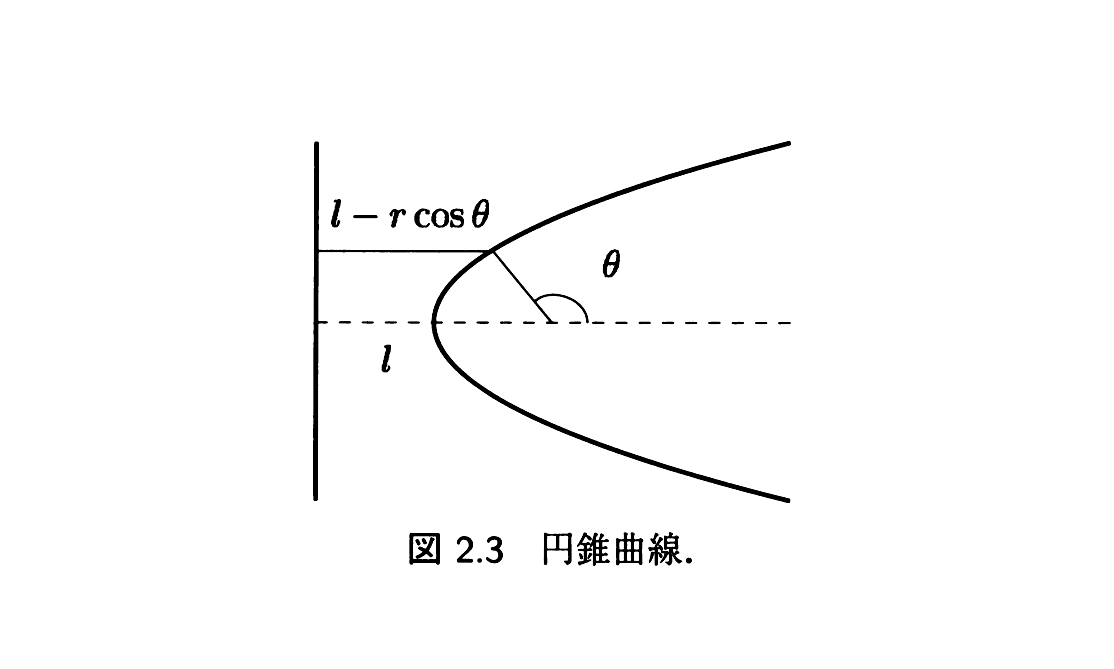
\includegraphics[width=0.50\textwidth,trim=0 32.88bp 0 0,clip]{figures/fig2.3.png}
  \figtitle{2.3}{圆锥曲线（原书 p.13）}
\end{figure}

由此得

\begin{equation}
  e = \frac{r}{l - r\cos\theta}
  \tag{2.1.52}
\end{equation}

如 图 2.3 所示，这是一条以 $e$ 为离心率（eccentricity）、以 $l$ 为从焦点
（focus）到准线（directrix）的距离（focal parameter）的圆锥曲线。

% [Tutor Note: 背景：Fermat 原理严格地说应表述为光程取驻值（一般并非最小），
% 原书此处作「最小」，译文照原书。]
\section{Lagrange 形式的分析力学}

直接用 Newton 运动定律写出运动方程，由于必须使用 Galilei 坐标系，往往很
麻烦。这在系统具有复杂约束条件时尤为显著。Lagrange 形式的分析力学通过用
变分原理（variational principle）改写运动定律，对这一问题给出优雅的处理
方法。

\subsection{变分原理}

用微分法可以求出函数的极值，而把它推广到无穷维，便成为变分法。变分原理
的滥觞是几何光学中的 Fermat 原理：

\fkstmt{Fermat 原理}{光沿光学距离最小的路径行进。}

设一非均匀介质充满 $\R^3$，其折射率由位置的函数 $n(\bm{x})$ 给出。把连接
两点 $p,q\in\R^3$ 的全部路径的集合记作

\begin{equation}
  \cP(p,q) = \{\,\gamma:[0,1]\to\R^3 \mid \gamma(0)=p,\ \gamma(1)=q\,\}
  \tag{2.2.1}
\end{equation}

这里，对路径 $\gamma:[0,1]\to\R^3$ 施加分段光滑等合理的条件。此时，路径
$\gamma$ 的距离由

\begin{equation}
  \ell[\gamma] = \int_0^1 \rd s
  \tag{2.2.2}
\end{equation}

给出。其中，把路径 $\gamma$ 用分量表示为
$\gamma(t) = (\gamma_x(t),\gamma_y(t),\gamma_z(t))$ 时，微线元 $\rd s$ 为

% [原文 p.14]
\begin{equation}
  \rd s = \sqrt{\Bigl(\frac{\rd\gamma_x}{\rd t}\Bigr)^2
    + \Bigl(\frac{\rd\gamma_y}{\rd t}\Bigr)^2
    + \Bigl(\frac{\rd\gamma_z}{\rd t}\Bigr)^2}\ \rd t
  \tag{2.2.3}
\end{equation}

所定义。把距离对应于各条路径的映射

\begin{equation}
  \ell : \cP \to \R
  \tag{2.2.4}
\end{equation}

是路径空间上的函数。每条路径自身又是函数 $\gamma:[0,1]\to\R^3$，所以 $\ell$
是「函数的函数」（即在由函数构成的空间上定义的函数）。一般把「函数的函数」
称为泛函（functional）。距离 $\ell$ 是泛函的典型例子。众所周知，连接 $\R^3$
中两点的最短路径由通过这两点的线段给出。

另一方面，光学距离由

\begin{equation}
  S[\gamma] = \int_0^1 n\,\rd s
  \tag{2.2.5}
\end{equation}

定义。例如，考虑这样的情形：不同的介质充满 $\R^3$ 内的上半空间
$\R^2\times\R^{>0}$ 与下半空间 $\R^2\times\R^{<0}$，而在边界 $\R^2\times 0$
处折射率不连续地变化。给定上半空间中的一点与下半空间中的一点时，在连接这
两点的分段光滑路径中，使光学距离 (2.2.5) 最小者，是由满足 Snell 法则

\begin{equation}
  n_1\sin\theta_1 = n_2\sin\theta_2
  \tag{2.2.6}
\end{equation}

的两条线段合并而成的集合。这里，$n_1$ 与 $n_2$ 分别是上半空间与下半空间中的
折射率，$\theta_1$ 与 $\theta_2$ 分别是上半空间与下半空间中的入射角。后来，
由 Foucault、Fizeau 等人开创的实验弄清了：折射率与介质中的光速成反比。因此，
Fermat 原理也可以改述为：光沿时间最短的路径行进。

\subsection{Euler--Lagrange 方程式}

固定流形 $W$、起始时刻 $t_0$、终止时刻 $t_1$，以及初始位置 $q_0\in W$ 与
终止位置 $q_1\in W$，考虑路径空间

\begin{equation}
  \cP = \{\,\gamma:[t_0,t_1]\to W \mid \gamma(t_0)=q_0,\ \gamma(t_1)=q_1\,\}
  \tag{2.2.7}
\end{equation}

上的泛函由 $W$ 的切丛（tangent bundle）$TW$ 上的函数
$L:TW\to\R$ 表示为

\begin{equation}
  S[\gamma] = \int_{t_0}^{t_1} L(\gamma,\dot\gamma)\,\rd t
  \tag{2.2.8}
\end{equation}

的情形。称 $W$ 为位形空间（configuration space），$L$ 为 Lagrange 函数
（Lagrangian），$S$ 为作用泛函（action functional）。取 $W$ 的局部坐标
$\varphi:U\to\R^n$，

% [原文 p.15]
记作

\begin{equation}
  \varphi\circ\gamma
    = \bm{q} = (q^1,\dots,q^n) : [0,1] \to \R^n
  \tag{2.2.9}
\end{equation}

对满足边界条件

\begin{equation}
  \delta\bm{q}(t_0) = \delta\bm{q}(t_1) = 0
  \tag{2.2.10}
\end{equation}

的任意函数 $\delta\bm{q}:[t_0,t_1]\to\R^n$，泛函的变分（variation）

\begin{equation}
  \delta S := S[\bm{q} + \delta\bm{q}] - S[\bm{q}]
  \tag{2.2.11}
\end{equation}

中关于 $\delta\bm{q}$ 的一次项为

\begin{align}
  \delta S &= \int_{t_0}^{t_1}
    \Bigl(\frac{\partial L}{\partial\bm{q}}\cdot\delta\bm{q}
      + \frac{\partial L}{\partial\dot{\bm{q}}}\cdot\delta\dot{\bm{q}}
    \Bigr)\rd t \tag{2.2.12}\\
  &= \Bigl[\frac{\partial L}{\partial\dot{\bm{q}}}\cdot\delta\bm{q}
    \Bigr]_{t_0}^{t_1}
    + \int_{t_0}^{t_1}
    \Bigl(\frac{\partial L}{\partial\bm{q}}\cdot\delta\bm{q}
      - \frac{\rd}{\rd t}\Bigl(\frac{\partial L}{\partial\dot{\bm{q}}}
      \Bigr)\cdot\delta\bm{q}\Bigr)\rd t \tag{2.2.13}\\
  &= \int_{t_0}^{t_1}
    \Bigl(\frac{\partial L}{\partial\bm{q}}
      - \frac{\rd}{\rd t}\Bigl(\frac{\partial L}{\partial\dot{\bm{q}}}
      \Bigr)\Bigr)\cdot\delta\bm{q}\,\rd t \tag{2.2.14}
\end{align}

这里用到了：由分部积分出现的边界项因边界条件 (2.2.10) 而消失。由变分法的
基本引理（fundamental lemma of calculus of variations），

\begin{equation}
  \int_{t_0}^{t_1} \bm{f}(t)\cdot\bm{g}(t)\,\rd t = 0
  \tag{2.2.15}
\end{equation}

对任意函数 $\bm{g}:\R\to\R^n$ 成立的必要充分条件是 $\bm{f}:\R\to\R^n$
恒等于 $0$，因此，为使 $S$ 的变分 $\delta S$ 对 $\bm{q}$ 的任意变分
$\delta\bm{q}$ 都为零，$\bm{q}$ 必须满足 Euler--Lagrange 方程式
（Euler--Lagrange equation）

\begin{equation}
  \frac{\partial L}{\partial\bm{q}}
    - \frac{\rd}{\rd t}\Bigl(\frac{\partial L}{\partial\dot{\bm{q}}}\Bigr)
    = 0
  \tag{2.2.16}
\end{equation}

在 Lagrange 形式的分析力学中，物理系统通过给出位形空间 $W$ 与 Lagrange
函数 $L:TW\to\R$ 来指定，系统的运动作为作用量的驻点，即变分 $\delta S$
为零的路径来实现。指定位形空间便确定了运动的舞台，而指定 Lagrange 函数则
同时确定了运动定律与力的定律。Lagrange 函数要这样来确定：使作用量的驻点
（即 Euler--Lagrange 方程的解）与观测到的实际运动相符；在简单情形下，用
系统的动能 $K$ 与势能 $V$ 表示为

\begin{equation}
  L = K - V
  \tag{2.2.17}
\end{equation}

% [原文 p.16]
\begin{remark}{2.2.1}
Lagrange 函数不必是切丛 $TW$ 上的函数，也可以考虑这样的理论（高阶微分
理论）：对大于 $2$ 的自然数 $k$，Lagrange 函数是 $k$ 阶 jet 丛
（$k$-th jet bundle）$J_kW$ 上的函数。但是，这样的理论这里不予讨论。
\end{remark}

这里，就前面举出的例子来看看 Lagrange 函数。

\begin{example}{2.2.2}
（简谐振动）$W=\R$，把 $TW\cong\R\times\R$ 的坐标记作 $(x,v)$ 时，
Lagrange 函数由

\begin{equation}
  L(x,v) = \frac{1}{2}mv^2 - \frac{1}{2}kx^2 - mgx
  \tag{2.2.18}
\end{equation}

给出。

\begin{align}
  \frac{\partial L}{\partial x} &= -kx - mg, \tag{2.2.19}\\
  \frac{\partial L}{\partial v} &= mv \tag{2.2.20}
\end{align}

因此，Euler--Lagrange 方程式为

\begin{equation}
  (-kx - mg) - \frac{\rd}{\rd t}(m\dot x) = 0
  \tag{2.2.21}
\end{equation}
\end{example}

\begin{example}{2.2.3}
（单摆）$W=S^1$，把 $TW\cong S^1\times\R$ 的坐标记作 $(\theta,\omega)$ 时，
Lagrange 函数由

\begin{equation}
  L(x,v) = \frac{1}{2}m(R\omega)^2 + mgR\cos\theta
  \tag{2.2.22}
\end{equation}

给出。

\begin{align}
  \frac{\partial L}{\partial\theta} &= -mgR\sin\theta, \tag{2.2.23}\\
  \frac{\partial L}{\partial\omega} &= mR^2\omega \tag{2.2.24}
\end{align}

因此，Euler--Lagrange 方程式为

\begin{equation}
  mgR\sin\theta + \frac{\rd}{\rd t}(R^2\dot\theta) = 0
  \tag{2.2.25}
\end{equation}

% [Tutor Note: 校勘：例 2.2.3、例 2.2.4 原书 Lagrange 函数均印作 $L(x,v)$，
% 按坐标应分别为 $L(\theta,\omega)$、$L(\bm{x}_1,\bm{x}_2,\bm{v}_1,\bm{v}_2)$；
% (2.2.25) 第二项按推导应含因子 $m$。均照录原文。]
\end{example}

\begin{example}{2.2.4}
（Kepler 问题）$W=\R^3\times\R^3$，把 $TW$ 的坐标记作
$(\bm{x}_1,\bm{x}_2,\bm{v}_1,\bm{v}_2)$ 时，Lagrange 函数由

\begin{equation}
  L(x,v) = \frac{1}{2}m_1|\dot{\bm{x}}_1|^2
    + \frac{1}{2}m_2|\dot{\bm{x}}_2|^2
    + \frac{m_1m_2}{|\bm{x}_1 - \bm{x}_2|}
  \tag{2.2.26}
\end{equation}

给出。重心的位置

% [原文 p.17]
\begin{equation}
  \bm{x}' = \frac{m_1\bm{x}_1 + m_2\bm{x}_2}{m_1 + m_2}
  \tag{2.2.27}
\end{equation}

与相对坐标

\begin{equation}
  \bm{x} = \bm{x}_1 - \bm{x}_2
  \tag{2.2.28}
\end{equation}

可以写出

\begin{align}
  \bm{x}_1 &= \frac{m_2}{m_1 + m_2}\,\bm{x} + \bm{x}', \tag{2.2.29}\\
  \bm{x}_2 &= -\frac{m_1}{m_1 + m_2}\,\bm{x} + \bm{x}'
  \tag{2.2.30}
\end{align}

因此，Lagrange 函数 (2.2.26) 可写作

\begin{equation}
  L = \frac{1}{2}\frac{m_1m_2}{m_1 + m_2}|\dot{\bm{x}}|^2
    + \frac{1}{2}(m_1 + m_2)|\dot{\bm{x}}'|^2
    + \frac{m_1m_2}{|\bm{x}|}
  \tag{2.2.31}
\end{equation}
\end{example}

% [Tutor Note: 难点：(2.2.31) 即二体问题分解为重心运动（质量 $m_1+m_2$、
% 坐标 $\bm{x}'$）与相对运动（约化质量、坐标 $\bm{x}$）两部分。]
\subsection{动量的守恒定律}

与 Newton 形式的力学相比，作为 Lagrange 形式分析力学的一个优点，来举出
动量的守恒定律。对某个 $i\in\{1,\dots,n\}$，Lagrange 函数 $L$ 不显含
$q^i$ 时，即

\begin{equation}
  \frac{\partial L}{\partial q^i} = 0
  \tag{2.2.32}
\end{equation}

成立时，称 $q^i$ 为循环坐标（cyclic coordinate）。此时，由
Euler--Lagrange 方程式立即得到

\begin{equation}
  \frac{\rd}{\rd t}\Bigl(\frac{\partial L}{\partial\dot q^i}\Bigr) = 0
  \tag{2.2.33}
\end{equation}

称

\begin{equation}
  p_i := \frac{\partial L}{\partial\dot q^i}
  \tag{2.2.34}
\end{equation}

为坐标 $q^i$ 的共轭动量（conjugate momentum）。(2.2.33) 表明：与循环坐标
共轭的动量守恒。某个坐标是循环坐标，意味着系统关于该坐标的平移不变。后面
将会说明，动量 $p_i$ 生成（generate）平移

\begin{equation}
\begin{aligned}
  q &= (q^1,\dots,q^{i-1},q^i,q^{i+1},\dots,q^n)\\
  &\mapsto q' = (q^1,\dots,q^{i-1},q^i + a,q^{i+1},\dots,q^n)
\end{aligned}
  \tag{2.2.35}
\end{equation}

从而，系统在该变换下不变，与这个动量守恒，二者等价。

\takeaway{运动是作用量的驻点；变分原理给出 Euler--Lagrange 方程，循环坐标对应动量守恒。}

% [原文 p.18]
\section{Legendre 变换}

向量空间 $V$ 上的函数 $f:V\to\R$ 为严格凸（strictly convex），是指对任意的
$v,w\in V$ 与 $t\in(0,1)$，有

\begin{equation}
  f((1-t)v + tw) < (1-t)f(v) + tf(w)
  \tag{2.3.1}
\end{equation}

成立。$\R^n$ 上的光滑函数 $f$ 为严格凸的必要充分条件是：Hesse 矩阵
（Hessian）$\mathrm{Hess}(f) = (\partial_i\partial_j f)_{i,j=1}^n$ 为正定
（即所有特征值均为正）。此时，映射

\begin{equation}
  \rd f : V\to V^*,\quad v\mapsto (\rd f)_v\in T_v^*V\cong V^*
  \tag{2.3.2}
\end{equation}

是单射。把这个映射用坐标写出，便是

\begin{equation}
  v\mapsto p = \frac{\partial f}{\partial v}
  \tag{2.3.3}
\end{equation}

把这个映射的逆映射记作 $v = v(\bm{p})$，称 $f$ 的 Legendre 变换
（Legendre transform）由

\begin{equation}
  f^* : V^*\to\R,\quad
  \bm{p}\mapsto \bm{p}\cdot\bm{v}(\bm{p}) - f(\bm{v}(\bm{p}))
  \tag{2.3.4}
\end{equation}

定义。此时，

\begin{align}
  \frac{\partial f^*}{\partial\bm{p}}
    &= \frac{\partial(\bm{p}\cdot\bm{v})}{\partial\bm{p}}
     - \frac{\partial f}{\partial\bm{v}}\cdot
       \frac{\partial\bm{v}}{\partial\bm{p}} \tag{2.3.5}\\
  &= \bm{v} + \bm{p}\cdot\frac{\partial\bm{v}}{\partial\bm{p}}
     - \frac{\partial f}{\partial\bm{v}}\cdot
       \frac{\partial\bm{v}}{\partial\bm{p}} \tag{2.3.6}\\
  &= \bm{v} \tag{2.3.7}
\end{align}

并且，

\begin{align}
  f^{**}(\bm{v}) &= \bm{v}\cdot\bm{p} - f^*(\bm{p}) \tag{2.3.8}\\
  &= \bm{v}\cdot\bm{p} - (\bm{p}\cdot\bm{v} - f(\bm{v}))
     \tag{2.3.9}\\
  &= f(\bm{v}) \tag{2.3.10}
\end{align}

即 Legendre 变换施行两次便回到原函数。

\takeaway{Legendre 变换用 $\rd f$ 的逆把 $v$ 换成 $p$；施行两次回到原函数。}

% [Tutor Note: 背景：取 $V=T_qW$、$f=L(q,\cdot)$，则 (2.3.4) 给出 Hamilton
% 函数 $H(q,p)=p\cdot\dot q-L(q,\dot q)$，$p=\partial L/\partial\dot q$ 即共轭动量。]
\section{Legendre--Fenchel 变换}

对 Legendre 变换更概念性的理解，由 Legendre--Fenchel 变换
（Legendre--Fenchel transform）给出。这是把 Legendre 变换推广到既不一定
凸、也不一定光滑的函数。对向量空间 $V$ 上的函数 $f:V\to\R$，其
Legendre--Fenchel 变换 $f^*:V^*\to\R$ 由如下方式定义：把 $\bm{p}\in V^*$ 映到

% [原文 p.19]
\begin{figure}[htbp]
  \centering
  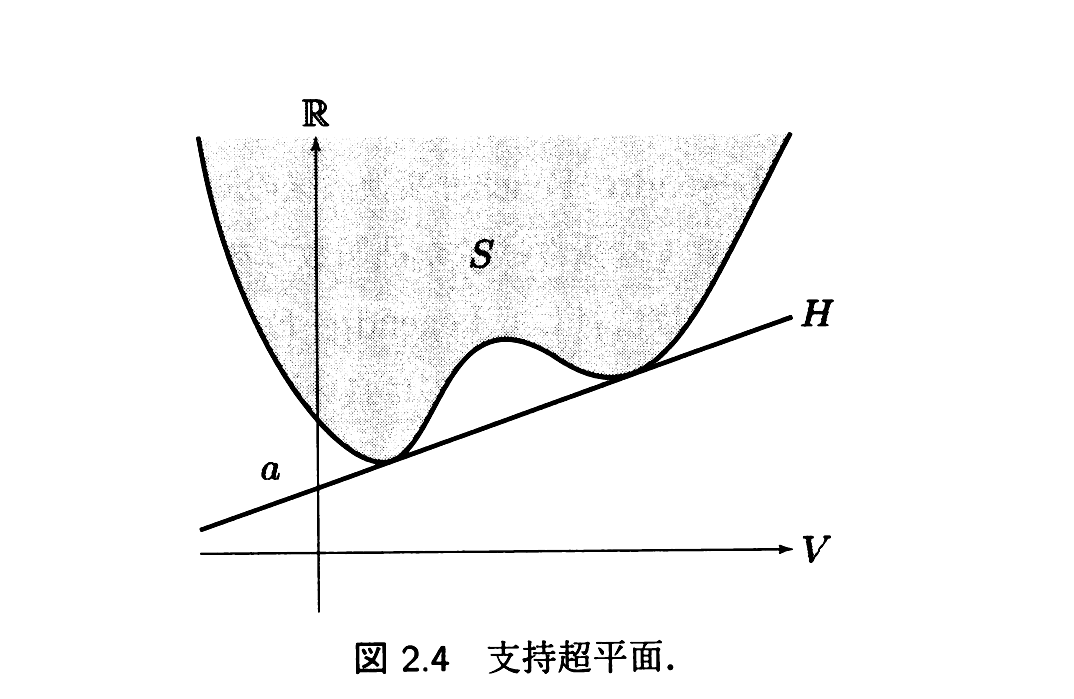
\includegraphics[width=0.50\textwidth,trim=0 14.16bp 0 0,clip]{figures/fig2.4.png}
  \figtitle{2.4}{支撑超平面（原书 p.19）}
\end{figure}

\begin{equation}
  f^*(\bm{p}) = \sup_{\bm{v}\in V}\bigl(\langle\bm{p},\bm{v}\rangle - f(\bm{v})\bigr)
  \tag{2.4.1}
\end{equation}

的映射。

对函数 $f$，定义 $V\times\R$ 的子集 $S$ 为

\begin{equation}
  S := \{\,(\bm{v},x)\in V\times\R \mid f(\bm{v})\le x\,\}
  \tag{2.4.2}
\end{equation}

集合 $S$ 的支撑超平面（supporting hyperplane）是指 $V\times\R$ 的超平面 $H$，
它与 $S$ 相交，并且 $V\times\R\setminus H$ 的两个连通分量中至少有一个不与
$S$ 相交。假设支撑超平面 $H$ 可表示为某个仿射函数

\begin{equation}
  g : V\to\R,\quad \bm{v}\mapsto \bm{p}\cdot\bm{v} + a
  \tag{2.4.3}
\end{equation}

的图像：

\begin{equation}
  H = \{\,(\bm{v},x)\in V\times\R \mid x = g(\bm{v})\,\}.
  \tag{2.4.4}
\end{equation}

其中，$\bm{p}\in V^*$ 是 $g$ 的斜率，$a$ 是 $g$ 在原点的值。由支撑超平面的
定义，存在某个 $\bm{v}_0\in V$，使

\begin{equation}
  f(\bm{v}_0) = g(\bm{v}_0) = \bm{p}\cdot\bm{v}_0 + a
  \tag{2.4.5}
\end{equation}

成立。对任意的 $\bm{p}\in V^*$，斜率为 $\bm{p}$ 的支撑超平面若存在则唯一。
包含 $S$ 的最小凸集称为 $S$ 的凸包（convex hull），记作 $\mathrm{Conv}(S)$。
具体地说，它是对 $S$ 的任意两点，把通过这两点的线段添加到 $S$ 而得到的：

\begin{equation}
  \mathrm{Conv}(S) = \{\,(1-t)p + tq \mid p,q\in S,\ t\in[0,1]\,\}.
  \tag{2.4.6}
\end{equation}

由定义显然，$S$ 的支撑超曲面全体的集合只依赖于 $S$ 的凸包。把此时的 $-a$
看作 $\bm{p}$ 的函数，就是 $f$ 的 Legendre--Fenchel 变换。对于这个
Legendre--Fenchel 变换，

\begin{itemize}
  \item 光滑凸函数的 Legendre--Fenchel 变换与 Legendre 变换一致；
% [原文 p.20]
  \item $f^*$ 必为凸函数；
  \item 由 Legendre--Fenchel 变换后的函数 $f^*$ 复原原函数 $f$ 的必要充分
    条件是 $f$ 为凸函数；
  \item 对凸函数把 Legendre--Fenchel 变换施行两次便回到原函数；
\end{itemize}

确认这些性质是很好的练习。

\takeaway{Legendre--Fenchel 变换取支撑超平面截距的负值；凸函数变换两次复原。}

\section{Hamilton 形式的分析力学}

Lagrange 函数具有

\begin{itemize}
  \item 是 $TW$ 上的函数（即只依赖于到路径的一阶微分）；
  \item 到 $TW$ 各纤维的限制是严格凸的；
\end{itemize}

这两条性质时，通过对 $TW$ 的各纤维作 Legendre 变换，便可由 Lagrange 函数
$L:TW\to\R$ 得到新的函数 $H:T^*W\to\R$。此时，称 $W$ 为位形空间
（configuration space），$T^*W$ 为相空间（phase space），$H$ 为
Hamilton 函数（Hamiltonian）。把 $W$ 的坐标记作 $\bm{q}$，把与 $\bm{q}$
对应的 $TW$ 及 $T^*W$ 的纤维方向坐标分别记作 $\bm{v}$ 与 $\bm{p}$，则
$L=L(\bm{q},\bm{v})$ 与 $H=H(\bm{q},\bm{p})$ 的关系由

\begin{equation}
  \bm{p} = \frac{\partial L}{\partial\bm{v}},\quad
  H(\bm{q},\bm{p}) = \bm{p}\cdot\bm{v}(\bm{q},\bm{p})
    - L(\bm{q},\bm{v}(\bm{q},\bm{p}))
  \tag{2.5.1}
\end{equation}

以及

\begin{equation}
  \bm{v} = \frac{\partial H}{\partial\bm{p}},\quad
  L(\bm{q},\bm{v}) = \bm{v}\cdot\bm{p}(\bm{q},\bm{v})
    - H(\bm{p}(\bm{q},\bm{v}),\bm{q})
  \tag{2.5.2}
\end{equation}

给出。由此，

\begin{align}
  \frac{\partial L}{\partial\bm{q}}
    &= \frac{\partial}{\partial\bm{q}}
       \bigl(\bm{v}\cdot\bm{p}(\bm{q},\bm{v})
         - H(\bm{p}(\bm{q},\bm{v}),\bm{q})\bigr) \tag{2.5.3}\\
  &= \bm{v}\cdot\frac{\partial\bm{p}}{\partial\bm{q}}
     - \frac{\partial H}{\partial\bm{p}}\cdot
       \frac{\partial\bm{p}}{\partial\bm{q}}
     - \frac{\partial H}{\partial\bm{q}} \tag{2.5.4}\\
  &= \bm{v}\cdot\frac{\partial\bm{p}}{\partial\bm{q}}
     - \bm{v}\cdot\frac{\partial\bm{p}}{\partial\bm{q}}
     - \frac{\partial H}{\partial\bm{q}} \tag{2.5.5}\\
  &= -\frac{\partial H}{\partial\bm{q}} \tag{2.5.6}
\end{align}

并且，$\bm{p}$ 与 $\bm{q}$ 的时间发展为

\begin{align}
  \frac{\rd\bm{p}}{\rd t}
    &= \frac{\rd}{\rd t}\Bigl(\frac{\partial L}{\partial\bm{v}}\Bigr)
     = \frac{\partial L}{\partial\bm{q}}
     = -\frac{\partial H}{\partial\bm{q}}, \tag{2.5.7}\\
  \frac{\rd\bm{q}}{\rd t}
    &= \bm{v} = \frac{\partial H}{\partial\bm{p}}, \tag{2.5.8}
\end{align}

即

\begin{equation}
  \frac{\rd\bm{p}}{\rd t} = -\frac{\partial H}{\partial\bm{q}},\qquad
  \frac{\rd\bm{q}}{\rd t} = \frac{\partial H}{\partial\bm{p}}
  \tag{2.5.9}
\end{equation}

% [原文 p.21]
从而可写成对称的形式。称 (2.5.9) 为 Hamilton 正则运动方程式
（Hamilton's canonical equation of motion）。

为了用变分原理改写运动方程式，把作用量改写为

\begin{align}
  S &= \int_{t_0}^{t_1} L(\bm{q},\dot{\bm{q}})\,\rd t \tag{2.5.10}\\
  &= \int_{t_0}^{t_1}
     \bigl(\bm{p}(\bm{q},\dot{\bm{q}})\cdot\bm{v}\,\rd t
       - H(\bm{p}(\bm{q},\dot{\bm{q}}),\bm{q})\,\rd t\bigr)
     \tag{2.5.11}\\
  &= \int_{t_0}^{t_1}
     \bigl(\bm{p}(\bm{q},\dot{\bm{q}})\cdot\rd\bm{q}
       - H(\bm{p}(\bm{q},\dot{\bm{q}}),\bm{q})\,\rd t\bigr)
     \tag{2.5.12}
\end{align}

此时 $p$ 仍是 $\bm{q}$ 与 $\dot{\bm{q}}$ 的函数；$S$ 是 $W$ 上路径所构成的空间

\begin{equation}
  \{\,\bm{q}:[t_0,t_1]\to W \mid \bm{q}(t_0)=\bm{q}_0,\
  \bm{q}(t_1)=\bm{q}_1\,\}
  \tag{2.5.13}
\end{equation}

上的函数。这里，忘掉 $\bm{p}$ 是 $\bm{q}$ 与 $\dot{\bm{q}}$ 的函数这一点，考虑
自由地取变分。也就是说，把 $S$ 看作在 $T^*W$ 上路径所构成的空间

\[
\begin{aligned}
  \bigl\{(\bm{q},\bm{p}):[t_0,t_1]\to T^*W \mid
  &(\bm{q}(t_0),\bm{p}(t_0)) = (\bm{q}_0,\bm{p}_0),\\
  &(\bm{q}(t_1),\bm{p}(t_1)) = (\bm{q}_1,\bm{p}_1)\bigr\}
\end{aligned}
\]

上定义的函数

\begin{equation}
  (\bm{q},\bm{p})\mapsto \int_{t_0}^{t_1}
  \bigl(\bm{p}\cdot\rd\bm{q} - H(\bm{q},\bm{p})\,\rd t\bigr)
  \tag{2.5.14}
\end{equation}

来取变分。于是，

\begin{align}
  \delta S &= \int_{t_0}^{t_1}
    \Bigl(\delta\bm{p}\cdot\rd\bm{q} + \bm{p}\cdot\rd(\delta\bm{q})
      - \Bigl(\frac{\partial H}{\partial\bm{p}}\cdot\delta\bm{p}
        + \frac{\partial H}{\partial\bm{q}}\cdot\delta\bm{q}\Bigr)\rd t
    \Bigr) \tag{2.5.15}\\
  &= \int_{t_0}^{t_1}
    \Bigl(\delta\bm{p}\cdot\rd\bm{q} - \rd\bm{p}\cdot\delta\bm{q}
      - \Bigl(\frac{\partial H}{\partial\bm{p}}\cdot\delta\bm{p}
        + \frac{\partial H}{\partial\bm{q}}\cdot\delta\bm{q}\Bigr)\rd t
    \Bigr) \tag{2.5.16}\\
  &= \int_{t_0}^{t_1}
    \Bigl(\Bigl(\frac{\rd\bm{q}}{\rd t}
        - \frac{\partial H}{\partial\bm{p}}\Bigr)\cdot\delta\bm{p}
      - \Bigl(\frac{\rd\bm{p}}{\rd t}
        + \frac{\partial H}{\partial\bm{q}}\Bigr)\cdot\delta\bm{q}
    \Bigr)\rd t \tag{2.5.17}
\end{align}

这里，从 (2.5.15) 移到 (2.5.16) 时，对第 2 项作了分部积分并舍去边界项：

\begin{equation}
  \int_{t_0}^{t_1}\bm{p}\cdot\rd(\delta\bm{q})
  = \bigl[\bm{p}\cdot\delta\bm{q}\bigr]_{t_0}^{t_1}
    - \int_{t_0}^{t_1}\rd\bm{p}\cdot\delta\bm{q}
  = -\int_{t_0}^{t_1}\rd\bm{p}\cdot\delta\bm{q}.
  \tag{2.5.18}
\end{equation}

由变分法的基本引理，为使 $\delta S = 0$ 对任意变分成立的必要充分条件是
Hamilton 正则运动方程式

\begin{equation}
  \frac{\rd\bm{q}}{\rd t} = \frac{\partial H}{\partial\bm{p}},\qquad
  \frac{\rd\bm{p}}{\rd t} = -\frac{\partial H}{\partial\bm{q}}
  \tag{2.5.19}
\end{equation}

% [Tutor Note: 难点：此处把 $\bm{p}$ 视为与 $\bm{q}$ 独立的变量（不再要求
% $\bm{p}=\partial L/\partial\dot{\bm{q}}$），这是相空间表述的关键一步。]
在 Lagrange 形式的分析力学中，
% [本 chunk 到此为止；该句续见 ch02b（原书 p.22）]
